\documentclass[10pt]{article}
\usepackage{amsmath,amsfonts,times}
\usepackage{graphicx,color,tikz}
\usepackage[paperwidth=15.6cm,paperheight=6.6cm,lmargin=0in,rmargin=0in,tmargin=0.in,bmargin=0.in]{geometry}
\usetikzlibrary{arrows.meta,calc,patterns}

% A cable in a box of air, in a cross-section: three regions (the air, the jacket, the core) over the outside.
% (a) The regions and their materials, and the pieces of surface between them.
% (b) A domain computing in the air and the jacket (two subdomains), the core excluded: the roles of the pieces.

\definecolor{cair}{rgb}{0.62,0.80,0.95}
\definecolor{cjacket}{rgb}{0.98,0.82,0.45}
\definecolor{ccore}{rgb}{0.85,0.50,0.25}
\definecolor{cbound}{rgb}{0.80,0.10,0.10}
\definecolor{cinter}{rgb}{0.10,0.45,0.15}

\tikzset{
  piece/.style={line width=1.4pt, draw=black},
  boundary/.style={line width=2.0pt, draw=cbound},
  interface/.style={line width=2.0pt, draw=cinter, densely dashed},
  lab/.style={font=\small, align=center, inner sep=1.5pt},
  key/.style={font=\small, anchor=west},
}

\begin{document}
\nopagecolor
\centering
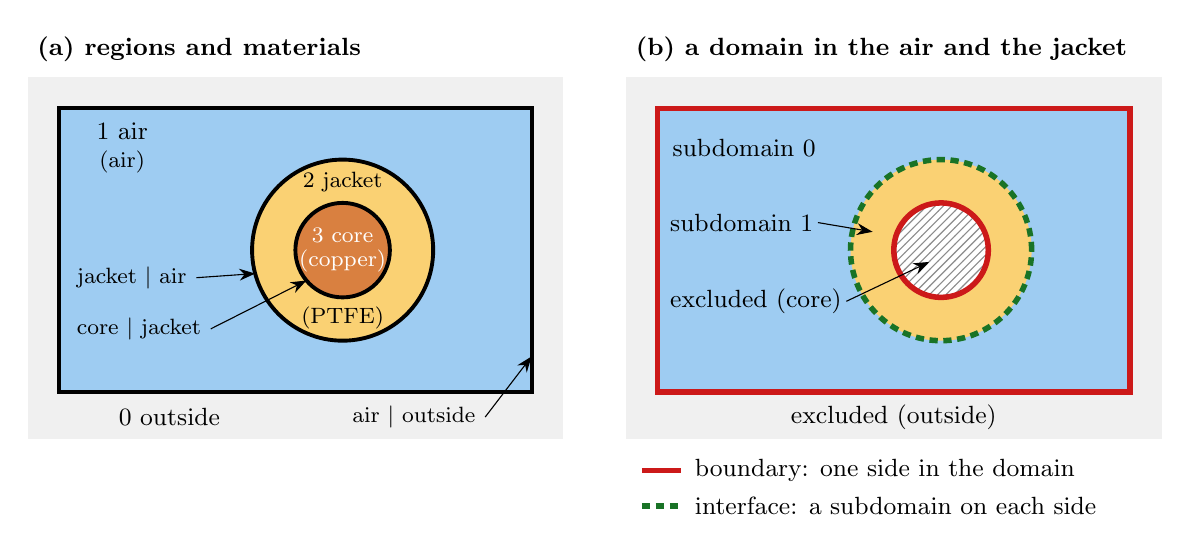
\begin{tikzpicture}[x=1cm, y=1cm]

  % (a) Regions and materials.
  \begin{scope}
    \node[font=\small\bfseries, anchor=west] at (-3.4,2.55) {(a) regions and materials};
    \fill[black!6] (-3.4,-2.4) rectangle (3.4,2.2);
    \fill[cair] (-3.0,-1.8) rectangle (3.0,1.8);
    \fill[cjacket] (0.6,0) circle (1.15);
    \fill[ccore] (0.6,0) circle (0.6);
    \draw[piece] (-3.0,-1.8) rectangle (3.0,1.8);
    \draw[piece] (0.6,0) circle (1.15);
    \draw[piece] (0.6,0) circle (0.6);
    \node[lab] at (-2.2,1.3) {1 air\\[-1pt]\footnotesize(air)};
    \node[lab] at (0.6,0.86) {\footnotesize 2 jacket};
    \node[lab] at (0.6,-0.86) {\footnotesize (PTFE)};
    \node[lab, text=white] at (0.6,0) {\footnotesize 3 core\\[-2pt]\footnotesize(copper)};
    \node[lab] at (-1.6,-2.12) {0 outside};
    \node[font=\footnotesize, anchor=west] (ja) at (-2.9,-0.35) {jacket $|$ air};
    \draw[-{Stealth[length=2mm]}] (ja.east) -- ($(0.6,0)+(195:1.15)$);
    \node[font=\footnotesize, anchor=west] (cj) at (-2.9,-1.0) {core $|$ jacket};
    \draw[-{Stealth[length=2mm]}] (cj.east) -- ($(0.6,0)+(220:0.6)$);
    \node[font=\footnotesize, anchor=west] (ao) at (0.6,-2.12) {air $|$ outside};
    \draw[-{Stealth[length=2mm]}] (ao.east) -- (3.0,-1.35);
  \end{scope}

  % (b) A domain over the same regions.
  \begin{scope}[shift={(7.6,0)}]
    \node[font=\small\bfseries, anchor=west] at (-3.4,2.55) {(b) a domain in the air and the jacket};
    \fill[black!6] (-3.4,-2.4) rectangle (3.4,2.2);
    \fill[cair] (-3.0,-1.8) rectangle (3.0,1.8);
    \fill[cjacket] (0.6,0) circle (1.15);
    \fill[white] (0.6,0) circle (0.6);
    \fill[pattern=north east lines, pattern color=black!45] (0.6,0) circle (0.6);
    \draw[boundary] (-3.0,-1.8) rectangle (3.0,1.8);
    \draw[interface] (0.6,0) circle (1.15);
    \draw[boundary] (0.6,0) circle (0.6);
    \node[lab] at (-1.9,1.3) {subdomain 0};
    \node[lab, anchor=west] (s1) at (-2.9,0.35) {subdomain 1};
    \draw[-{Stealth[length=2mm]}] (s1.east) -- ($(0.6,0)+(165:0.9)$);
    \node[lab, anchor=west] (ex) at (-2.9,-0.65) {excluded (core)};
    \draw[-{Stealth[length=2mm]}] (ex.east) -- (0.45,-0.15);
    \node[lab] at (0,-2.12) {excluded (outside)};
  \end{scope}

  % Key for (b).
  \begin{scope}[shift={(4.4,-2.8)}]
    \draw[boundary] (0,0) -- (0.5,0);
    \node[key] at (0.55,0) {boundary: one side in the domain};
    \draw[interface] (0,-0.45) -- (0.5,-0.45);
    \node[key] at (0.55,-0.45) {interface: a subdomain on each side};
  \end{scope}

\end{tikzpicture}
\end{document}
